%% ===================================================================
%% PART IV
%% ===================================================================
\part{Examples, classification and consequences}

%% -------------------------------------------------------------------
\section{The explicit rank-three obstruction}\label{sec:E4}

\subsection{The even-weight code of length four}

Let $C=E_4=\{w\in\F_2^4:\ \wt(w)\ \text{even}\}$, the kernel of $M=(1\,1\,1\,1)$; $k=3$. We write words by their supports, e.g.\ $13$ for $\{1,3\}$.

\paragraph{Circuits.} The six weight-two words $12,13,14,23,24,34$ (Proposition~\ref{prop:Emin}); $1234$ is not a circuit. Pairs of disjoint circuits: $\{12,34\}$, $\{13,24\}$, $\{14,23\}$. So $\Part=\{P_1,P_2,P_3\}$ with $P_1=\{12,34\}$, $P_2=\{13,24\}$, $P_3=\{14,23\}$, and $n_2=3$, $m_P=2$ for all three. The counting identity reads $3\cdot(2^2-2)=6=2^3-2$.

\paragraph{Cells.} The fibre is $F=\{12,13,14,23,24,34,1234\}$ (seven points). A direct enumeration from Definition~\ref{def:cell} gives $7$ vertices, $18$ edges ($6$ circuits $\times$ $3$ admissible cosets) and exactly $3$ two-dimensional cells:
\begin{align*}
Z_A&=Z(\{12,34\},13)\quad\text{vertices }13,\,14,\,23,\,24,\\
Z_B&=Z(\{13,24\},12)\quad\text{vertices }12,\,14,\,23,\,34,\\
Z_C&=Z(\{14,23\},12)\quad\text{vertices }12,\,13,\,24,\,34.
\end{align*}
Their unions are all $\{1,2,3,4\}$, there is nothing outside the union, and the three centres are $(\tfrac12,\tfrac12,\tfrac12,\tfrac12)$ (Theorem~\ref{thm:centre}). Hence all three pairs collide. The cells $Z_A,Z_B$ share the diagonal with endpoints $14$ and $23$; $Z_A,Z_C$ share $13,24$; $Z_B,Z_C$ share $12,34$. The cell structure is the three equatorial squares of the octahedron with vertices $12,13,14,23,24,34$, together with the vertex $1234$ and edges to it (Figure~\ref{fig:octa}).

\paragraph{The rank.} With the common base point $x=14$ (not in $\spn P_1=\{0,12,34,1234\}$ nor in $\spn P_2=\{0,13,24,1234\}$), $s=(1-2x_i)_i=(-1,1,1,-1)$ and
\[
g_1=(-1,1,0,0),\ g_2=(0,0,1,-1);\qquad h_1=(-1,0,1,0),\ h_2=(0,1,0,-1).
\]
Then $g_1+g_2=(-1,1,1,-1)=h_1+h_2$. The vectors $g_1,g_2,h_1$ are independent: a relation $ag_1+bg_2+ch_1=0$ gives from coordinate~$2$ that $a=0$, from coordinate~$4$ that $b=0$ and then $c=0$. So the witness rank is exactly $3$. Because $r=t=2$, the witness space has dimension $3=r+t-1$. By Lemma~\ref{lem:LOW} no collision of $E_4$ has smaller rank; by Theorem~\ref{thm:rank3} the same is true of every non-embedded box.

\begin{remark}[Geometry of the witness]
The three planes in $\R^4$ spanned by $Z_A,Z_B,Z_C$ lie in the common affine hyperplane $\sum x_i=2$, which is $3$-dimensional. In that $\R^3$ the octahedron is a genuine picture: two equatorial squares meet along a diagonal and a third square passes through the common centre. The collision is thus a ``crossing of two planes in a $3$-space'', the simplest possible crossing.
\end{remark}

\subsection{Minimality and uniqueness}

\begin{proposition}\label{prop:unique-k3}
$E_4$ is minimal (Proposition~\ref{prop:Emin}). Every minimal non-embedded box of nullity $3$ is a blow-up of $E_4$ (that is, $p=4$ and $X=\AG(2,2)$).
\end{proposition}

\begin{proof}
For $k=3$ the affine space $H=\AG(2,2)$ has four points, so $p\le4$, and $p\ge k+1=4$ gives $X=H$; the code is $\mathrm{RM}(1,2)=E_4$.
\end{proof}

\subsection{Higher nullity}

\paragraph{Reed--Muller family.} By Proposition~\ref{prop:RM}, for every $k\ge3$ the box $\mathrm{RM}(1,k-1)$ of length $2^{k-1}$ is minimal non-embedded, with $2^{k-1}-1$ two-circuit partitions of $\one$ into complementary pairs of weight $p/2$. For $k=4$ ($n=8$): circuits are the $14$ words of weight $4$; the rank-three collision uses any two of the seven partitions. For $k=3$ it is $E_4$.

\paragraph{Blow-ups.} Replacing coordinate $i$ of $E_4$ by $\mu_i\ge1$ copies gives minimal boxes of every length $n\ge4$ and nullity $3$ (Proposition~\ref{prop:series}); all have $\rmin=3$.

\paragraph{Beyond Reed--Muller.} The minimal reduced box with $k=4$, $p=6$ has point set (coordinates $1,\dots,6$)
\[
X=\{1000,1001,1010,1011,1100,1101\}\subset\AG(3,2),
\]
$11$ circuits, and the five partitions of $\one$ shown in Figure~\ref{fig:twopart}: the four two-block partitions $\{135|246\}$, $\{235|146\}$, $\{145|236\}$, $\{245|136\}$ and the three-block partition $\{12|34|56\}$. The identity $4\cdot2+6=14=2^4-2$ holds, as does Parseval's identity (Example~\ref{ex:parseval}). A rank-three collision comes from any two of the four two-block partitions. The class with $k=5$, $p=8$ has two-block partitions (eight of them) and one four-block partition $\{12|34|56|78\}$, with $8\cdot2+14=30$.

\begin{remark}[Individual versus minimum, again]
Exact enumeration shows that the $k=4$, $p=6$ box has $78$ collisions ($66$ between cells of dimensions $(2,2)$ and $12$ between $(2,3)$), of witness rank $3$ ($30$ times) and $4$ ($48$ times); the $k=5$, $p=8$ box has $1596$ collisions ($1540$ of type $(2,2)$ and $56$ of type $(2,4)$) with ranks $3,4,5$ occurring $364,1176,56$ times. The theorem concerns the \emph{minimum}.
\end{remark}

%% -------------------------------------------------------------------
\section{Exact finite classification}\label{sec:classify}

This section reports the classification of minimal reduced boxes for small nullity. It is \emph{not used} in the proof of Theorem~\ref{thm:rank3}; its role is to document the examples, to provide independent evidence for the general theorems, and to record what is known beyond them.

\subsection{What is classified}

By Theorem~\ref{thm:affine} and Proposition~\ref{prop:series}, a minimal non-embedded box is determined, up to coordinate permutation and basis change, by (i)~its nullity $k$, (ii)~a spanning subset $X\subseteq\AG(k-1,2)$ up to $\AGL(k-1,2)$, and (iii)~a multiplicity function $\mu:X\to\Z_{\ge1}$. So classifying minimal boxes of nullity $k$ means classifying the $\AGL(k-1,2)$-orbits of subsets $X$ whose reduced box is minimal non-embedded; call these \emph{minimal classes}.

\subsection{Results}

\begin{table}[ht]
\centering\small
\begin{tabular}{@{}rrrp{6.2cm}@{}}
\toprule
$k$ & minimal classes & $p$ range & status and provenance\\
\midrule
$3$ & $1$ & $4$ & \PROVED+\CHECKED; re-enumerated here\\
$4$ & $3$ & $6,7,8$ & \PROVED+\CHECKED; re-enumerated here ($37$ labelled subsets)\\
$5$ & $12$ & $8,\dots,16$ & \PROVED+\CHECKED; re-enumerated here ($19\,373$ labelled subsets)\\
$6$ & $215$ & $10,\dots,32$ & source-reported (\gid{G10-T4}); the $215$ representatives were re-checked here; completeness not re-derived\\
\bottomrule
\end{tabular}
\caption{Minimal classes of reduced boxes by nullity. ``Re-enumerated'' means that all $2^{2^{k-1}}$ subsets of $\AG(k-1,2)$ were examined with the independent engine of Appendix~\ref{app:repro} (no use of the release code).}\label{tab:classes}
\end{table}

\begin{theorem}[Classification for $k\le5$; \gid{G8-T3b}, \gid{G9-T4}]\label{thm:class35}
The minimal reduced boxes with $k=3,4,5$ form $1$, $3$ and $12$ classes respectively, listed in Table~\ref{tab:classlist}. Each has $n_2\ge p-1$ whenever $p\ge9$ and $n_2\ge3$ always; each satisfies the counting and Parseval identities; all have $\rmin=3$.
\end{theorem}

\begin{proof}
The proof is an exhaustive enumeration. For each $k\in\{3,4,5\}$ every subset $X\subseteq\AG(k-1,2)$ with $|X|\ge k+1$ that spans $\F_2^k$ ($1$, $93$ and $57\,541$ subsets) was tested: non-embeddedness by Theorem~\ref{thm:E1} (enumeration of circuit partitions) and minimality by Definition~\ref{def:minimal} (shortening at each of the $p$ coordinates). The minimal subsets ($1$, $37$, $19\,373$) were grouped into $\AGL(k-1,2)$-orbits by closing under the generators of $\AGL(k-1,2)$ (translations and elementary transvections); the orbit counts are $1$, $3$, $12$, and the orbit sizes $1$; $28,8,1$; $840,4480,6720,448,1680,2688,140,1680,560,120,16,1$ add up to the numbers of subsets above.
\end{proof}

\src{\gid{G8-T3b} (nullity $3,4$, v008 \texttt{MINIMAL\_RANK.md}) and \gid{G9-T4} (nullity $5$, v009 \texttt{MATHEMATICS.md} \S2.2), both \PROVED+\CHECKED in the source. The enumeration here is independent of the release code; counts agree. The classification for nullity $5$ in the source lists $p=8,9,10,10,11,11,12,12,13,14,15,16$; so does Table~\ref{tab:classlist}.}

\begin{table}[ht]
\centering\small
\begin{tabular}{@{}rrrlrr@{}}
\toprule
$k$ & $p$ & $n_2$ & profile $m^{n_m}$ & orbit size & $|\mathrm{Stab}|$\\
\midrule
\classtablebody
\bottomrule
\end{tabular}
\caption{The $16$ minimal classes of nullity $3,4,5$. ``Profile'' lists the number $n_m$ of partitions of $\one$ with $m$ blocks. ``Orbit size'' is the number of labelled subsets of $\AG(k-1,2)$ in the class; $|\mathrm{Stab}|=|\AGL(k-1,2)|/\text{orbit size}$ ($24$, $1344$, $322\,560$ for $k=3,4,5$). Exact output of \texttt{scripts/classify.py}.}\label{tab:classlist}
\end{table}

\paragraph{Burnside counts.} The number of $\AGL(m,2)$-orbits on all subsets of $\AG(m,2)$ (including $\emptyset$) is $5,10,32$ for $m=2,3,4$ (group orders $24,1344,322\,560$; computed here by Burnside's lemma with exhaustively generated groups) and $382$ for $m=5$ (source-reported). For $k=m+1=6$ this gives the source's chain of counts: $381$ non-empty orbits, $350$ spanning, $349$ non-embedded, $215$ minimal.

\begin{theorem}[Nullity six; \gid{G10-T4}, source-reported]\label{thm:class6}
There are $215$ minimal classes of reduced boxes with $k=6$, with $10\le p\le32$ and $16\le n_2\le31$. Every class has W2, rank $3$, satisfies the identities, and $n_2\ge p-1$ when $p\ge9$ holds in all cases.
\end{theorem}

\src{\gid{G10-T4}, GEO-I v010 \texttt{BINARY6.md} (\PROVED+\CHECKED: certificates \texttt{C6\_rank6.json} with the checker \texttt{checker10.py}). \emph{Independent verification here:} the list of $215$ representative supports was read from the certificate file and, with the independent engine, each was confirmed to be a minimal non-embedded reduced box, to satisfy the counting and Parseval identities and $n_2\ge p-1$ ($p\ge9$), and to have the recorded $n_2$; the $215$ supports are pairwise inequivalent under $\AGL(5,2)$ (separated by invariants, with an exhaustive backtracking search for the $8$ pairs sharing invariants). \emph{Not re-derived:} that the list is complete. Distribution of $(p,n_2)$ in Table~\ref{tab:ksix}.}

\begin{table}[ht]
\centering\small
\begin{tabular}{@{}rrrr@{}}
\toprule
$p$ & classes & $\min n_2$ & $\max n_2$\\
\midrule
\ksixtablebody
\bottomrule
\end{tabular}
\caption{Nullity six: the $215$ source-reported classes, recomputed with the independent engine (\texttt{scripts/verify6.py}).}\label{tab:ksix}
\end{table}

\begin{figure}[ht]
\centering
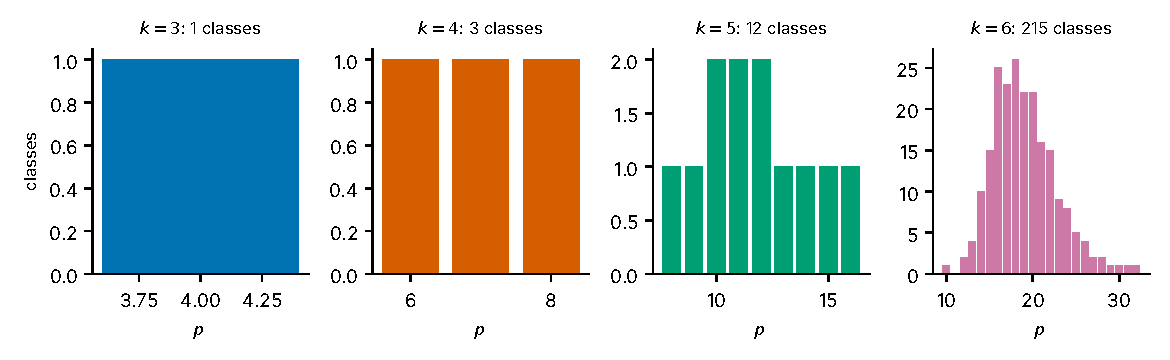
\includegraphics[width=0.95\textwidth]{figures/fig12_classification.pdf}
\caption{Classification summary for $k=3,\dots,6$: number of minimal classes by reduced length $p$. \figdesc{exact counts; $k=6$ from the source-reported list recomputed here.}}\label{fig:classes}
\end{figure}

\subsection{Algorithms and certificates}

\paragraph{Enumeration algorithm ($k\le5$).} For every subset $X$ of $\AG(k-1,2)$ (as a bitmask of the $2^{k-1}$ points): (1)~discard it unless it has rank~$k$ and $p\ge k+1$; (2)~compute all $2^k-1$ nonzero words and their circuits (inclusion-minimal supports); (3)~enumerate all families of pairwise disjoint circuits and record which unions have two partitions (Theorem~\ref{thm:E1}); (4)~for each coordinate $i$ repeat (3) on the circuits avoiding $i$ (Lemma~\ref{lem:shortcirc}); (5)~$X$ is minimal iff (3) finds a double partition and (4) never does. Orbits: union--find over the generators of $\AGL(k-1,2)$.

\paragraph{Certificates.} A \emph{partition certificate} for a point set $X\subseteq\AG(k-1,2)$ consists of the points and two functionals $f\ne g$ whose words are disjoint circuits covering $X$, together with a second such pair; a standalone checker confirms it using only rank computations (source format PARTITION, \texttt{checker11.py}). By Theorems~\ref{thm:E1} and~\ref{thm:L5} a valid certificate proves non-embeddedness with a rank-three collision. It does \emph{not} certify minimality. All $231$ source certificates (every minimal class with $k\le6$) were accepted by the unchanged source checker and, independently, by the engine here.

\paragraph{Separation of roles.} The classification is a table of examples. The universal theorems in Part~III do not depend on it: W2 for $p\ge9$ is proved by inequality, W2 for $p\le8$ by a different small enumeration (Section~\ref{sec:W2}), and Theorem~\ref{thm:rank3} follows.

\subsection{Historical statuses}

Several statements recorded in the release series were later settled; their current status is recorded here for completeness (details in Appendix~\ref{app:crosswalk}): \gid{G8-C3} (full support of minimal boxes) was open in v008--v009 and is proved as Theorem~\ref{thm:F1}; \gid{G10-C1} (universal $\rmin=3$) was open in v010 and is Theorem~\ref{thm:rank3}; \gid{G10-C2} (existence of a rank-four minimal box) is \textsc{false} (Corollary~\ref{cor:no4}); the v010 implication ``$\rmin\ge4$ requires nullity $\ge7$'' is vacuous.

\begin{question}[Spanning sets]\label{q:spanning}
Is the box of every spanning subset $X\subseteq\AG(k-1,2)$ with $|X|\ge k+1$ non-embedded? This holds for $k\le5$ in the exhaustive enumeration here, for $k=6$ in the source counts ($350$ spanning orbits, $349$ non-embedded; the one exceptional orbit is presumably the simplex $p=k$, for which $C=\F_2^k$ is embedded, but we have not checked this against the source enumeration), and in all of $540$ random samples with $k\in\{6,7,8\}$, $p-k\in\{2,3,4\}$ tested here. It is not proved.
\end{question}

%% -------------------------------------------------------------------
\section{Implications}\label{sec:implications}

\subsection{Uniform obstruction dimension}

Theorem~\ref{thm:rank3} says that the \emph{obstruction to embeddedness has a uniform local size}: every non-embedded box, of any length $n$ and nullity $k$, contains a pair of $2$-dimensional cells in a common $3$-dimensional affine subspace whose relative interiors cross at their centres. In geometric language: non-embedding never needs a configuration of higher dimension than the crossing of two planes in $3$-space. The ambient dimension $n$ may be arbitrarily large, and $\spn$ of all cells may be $n$-dimensional, but the obstruction is already visible in dimension three.

\begin{corollary}[A short certificate]\label{cor:cert}
A box $C$ is non-embedded if and only if it contains a word $a$ with two distinct decompositions $a=b_1\sqcup b_2=c_1\sqcup c_2$ into two disjoint circuits.
\end{corollary}

\begin{proof}
($\Leftarrow$)~Theorem~\ref{thm:L5}. ($\Rightarrow$)~By Proposition~\ref{prop:descent} and Theorem~\ref{thm:W2} there is a minimal sub-box $C_{(I)}$ with two two-circuit partitions of its all-ones word; their circuits are circuits of $C$ (Lemma~\ref{lem:shortcirc}), and $a=\one_{[n]\setminus I}$ is a word of $C$ with two decompositions.
\end{proof}

\subsection{Rigidity, finite affine structure, partition universality}

\emph{Rigidity.} In a minimal box the circuit structure is determined by a single failure of unique decomposition (Theorem~\ref{thm:rigid}); the number of cells at the centre is $\sum_P(2^{k-m_P}-1)$ (Proposition~\ref{prop:centre-count}); for example $E_4$ has $3$, the $k=4$, $p=6$ box has $13$, $\AG(3,2)$ has $21$, the $k=5$ classes have $57,69,87,105$ for $p=8,9,10,10$ (verified by direct enumeration).

\emph{Finite affine structure.} Minimal boxes are exactly (up to blow-up) the subsets $X\subseteq\AG(k-1,2)$ whose code has the rigidity property of Proposition~\ref{prop:rigid-char}. The problem of classifying all minimal boxes becomes the problem of classifying certain subsets of affine spaces over $\F_2$ up to the affine group.

\emph{Partition universality.} Every minimal box carries a vector-space partition of $\F_2^{k-1}$ built from its circuit partitions, satisfying the counting identity and the Parseval identity; at least $p-1$ of its parts (for $p\ge9$) are one-dimensional.

\subsection{Local witness versus global complexity}

\begin{remark}[What rank three does and does not give]\label{rem:algo}
Corollary~\ref{cor:cert} gives a certificate of non-embeddedness of size $O(n)$ (five subsets of $[n]$): the verification that $b_1,b_2,c_1,c_2$ are circuits of $C$ summing to the same word requires only rank computations of column submatrices of $M$ (a set $T$ is a circuit iff the columns of $M$ indexed by $T$ have a one-dimensional kernel spanned by $\one_T$). So non-embeddedness has polynomially checkable certificates in the binary-matrix encoding. This does \textbf{not} yield a polynomial-time \emph{algorithm}: the theorem asserts the existence of such a word but not how to find it, and the number of candidates for $a$ is exponential in $n$. We make no claim about the computational complexity of deciding embeddedness; and ``bounded witness rank'' must not be read as ``efficient detection''. The size of the local witness is uniformly $3$; the cost of locating it is unaddressed.
\end{remark}

\subsection{Consequences for the arithmetic model}

Within the arithmetic setting of the GEO-I series the binary boxes arise as the $0/1$ slices of congruence lattices. The theorem implies that, whenever a binary relation lattice (for a given set of active primes and parity configuration) has an exceptional cell overlap, that overlap already occurs in a $3$-dimensional exponent subspace and is generated by exactly two pairs of $2$-dimensional moves. Whether a particular arithmetic fibre is of this binary type is a separate question (Remark~\ref{rem:realize}), which this paper does not address.
